\documentclass{IEEEtran}
\usepackage{graphicx}



\begin{document}

\title{Homework 3: Broadcast, Reduce and AllReduce}
\author{Brandon Bell}
%\markboth{Brandon}{HW 2}
\maketitle
\begin{abstract}
HW3 is an introduction to various methods of using tree style communication between processes. Tree communication is a generally much more efficient method of disseminating or collecting data among process as it scales as O(Log(p)). The goal of HW3 is to hand code versions of MPI’s Broadcast, Reduce, and All Reduce functions using C’s bit-wise operators for controlling the communication tree’s structure.
\end{abstract}



\section{Tree Structured Broadcast and Reduce}
 \begin{figure}
        \center{\includegraphics
        {fig1.ps}}
        \caption{\label{Broadcast} Low to high bit broadcast for 4 nodes.
\end{figure}


\section{Trapezoidal Rule Integration With Linear Reduce}
I simply modified the all the one reduction method of the original Trapezoidal Rule code from the books source code to use a linear reduce. The highest ranked process (p) starts the reduce by sending the to total of it’s integration region to process (p-1) which, then adds the total of process p to it’s own and send the new running total to process (p-2) and so until p0. Process 0 receives the running total, adds it’s region to the total and prints the results. I think this linear reduce is is about as efficient as the orginal all-to-one reduce as they are both scale as O(P). However, in this regime of small latency dominated messages, I think that there may be a small advantage to the all-to-one reduce since the overhead of sending a message is palatalized. When run with 8 processes my program finds,

\begin{verbatim}
% mpirun -n 8 ./HW2-Part2 
With n = 1024 trapezoids, our estimate 
of the integral from 0.000000 
to 1.000000 = 0.333333
\end{verbatim}

which agrees with the finding of the original program when run with 8 processes.

\begin{verbatim}
% mpirun -n 8 ./get_data  
Enter a, b, and n 
0 1 1024 
With n = 1024 trapezoids, our estimate 
of the integral from 0.000000 
to 1.000000 = 0.333333
\end{verbatim}

\section{Simpson's Rule}
I started out by writing a serial version of Simpson’s Rule with a fixed function of $f(x) = x^{2}$, fixed region of integration [0,1], and a fixed number of intervals, 1024.  My implementation of Simpsons Rule.

\begin{verbatim}
    // Take care of the starting and end points. 
 2    integral = f(a) + f(b); 
 3    // Loop through the n strips in the region. 
 4    for ( int i=1; i<(2*n - 1); i++ ) 
 5    { 
 6 // increment x by a half interval at a time.
 7         x += h / 2; 
 8         if ( i % 2 == 0 ) 
 9             integral += ( 2 * f(x) ); 
10         else  
11             integral += ( 4 * f(x) ); 
12    } 
13    integral *= ( h / 3 );
\end{verbatim}

Then to serialize this implementation, I worked this integration function into the the linear reduce version of the Trapezoidal rule code from part 2. 

This parallel Simpson’s Rule code also incorporates command line arguments to set the number of intervals used and and to print out the interval partition assigned to each process. All of the output is handled by process 0 but, all the processes are aware of any arguments given.  This implementation of Simpson's Rule requires that the number of intervals be even so, the code checks the parity of a user defined interval number and if it’s odd, the code increments it by one to make it even and then carries on with the new even interval count. If the interval value entered is not a valid base 10 int value a warning is issued about incorrect arguments, command line argument parsing stops and the program carries on with the hard coded interval count of 1024. Each process determines a new interval count from the command line arguments, if present, so no time consuming message passing is required. 

To implement the verbose option to print out the interval coefficients being handled by each process, process 0 calculates the partition scheme from the variable of integration and does not depend of communication from the other processes. At present my code has process 0  do this calculation after it has received the total from all the other process. It would probably be more optimal the partitions where determined and and output while process 0 was waiting for the linear reduce to complete, thereby reducing idle process time, but the difference would be minimal at this level I expect. There is a known bug that i've been unabel to track down, setting -v before -i results in the new interval value being read as 0 regardless of specified value. In the case that an interval of 0 is found the code falls back to the hard coded value of 1024.

Examples:

\begin{verbatim}
% mpirun -n 4 ./HW2-Part3-Parallel         
With n = 1024 intervals, our estimate
of the integral from 0.000000 to 1.000000 = 0.664229

% mpirun -n 4 ./HW2-Part3-Parallel -i 11
With n = 12 intervals, our estimate
of the integral from 0.000000 to 1.000000 = 0.480710

% mpirun -n 4 ./HW2-Part3-Parallel -i 11 -v
Process 0: [ 1 4 2 ]
Process 1: [ 2 4 2 ]
Process 2: [ 2 4 2 ]
Process 3: [ 2 4 1 ]
With n = 12 intervals, our estimate
of the integral from 0.000000 to 1.000000 = 0.480710

mpirun -n 8 ./HW2-Part3-Parallel -i 36 -v
Process 0: [ 1 4 2 4 ]
Process 1: [ 2 4 2 4 ]
Process 2: [ 2 4 2 4 ]
Process 3: [ 2 4 2 4 ]
Process 4: [ 2 4 2 4 ]
Process 5: [ 2 4 2 4 ]
Process 6: [ 2 4 2 4 ]
Process 7: [ 2 4 2 1 ]
With n = 36 intervals, our estimate
of the integral from 0.000000 to 1.000000 = 0.379001

\end{verbatim}

\end{document}
